\documentclass[11pt]{article}
\usepackage[margin=2.9cm]{geometry}
\usepackage{amsmath,amssymb,amsthm}
\usepackage{graphicx}
\usepackage{booktabs}
\usepackage[hidelinks]{hyperref}
\usepackage{xeCJK}
\setCJKmainfont{Hiragino Mincho ProN}

% ---- named theorem environments (labels match the internal claim tree) ----
\newtheorem{innerthm}{Theorem}
\newenvironment{namedthm}[1]{\par\medskip\noindent\textbf{#1.}\itshape}{\par\medskip}
\newenvironment{namedprop}[1]{\par\medskip\noindent\textbf{#1.}\itshape}{\par\medskip}
\newtheorem{lemma}{Lemma}
\newtheorem{remark}{Remark}
\newtheorem{conjecture}{Conjecture}

\newcommand{\dd}{\,\mathrm{d}}
\newcommand{\E}{\mathbb{E}}
\newcommand{\PP}{\mathbb{P}}
\newcommand{\R}{\mathbb{R}}
\newcommand{\Kmix}{K_{\mathrm{mix}}}
\newcommand{\Ts}{T_s}
\newcommand{\Ta}{T_a}
\newcommand{\Tg}{T_g}
\newcommand{\relL}{\bar\Lambda}
\newcommand{\wbar}{\bar w}

\title{Contact processes on ballistic Poisson particles:\\
criticality, fronts, and when motion helps colonization\\[1ex]
\large (Preprint --- Zenodo v1)}
\author{Yukie Maeda\thanks{Independent researcher. The role of AI systems in this
work is disclosed in Section~\ref{sec:verification} and Appendix~B.}}
\date{August 2026}

\begin{document}
\maketitle

\begin{abstract}
\noindent\textbf{和文要旨.}
実測恒星運動学を動機として、等速直線運動する Poisson 粒子系上の接触過程
$M(\rho,\nu,R,p,\tau,\Ts)$(進入駆動・撃ちっ放し・対一回・再マーク許可)を導入し、
その臨界構造を確立する。主結果: (i) 転送核のスペクトル条件 $r(K)<1$ による絶滅定理
(定理A)、(ii) この SIR 型分枝上界は再マーク許可の完全モデルには拡張されないこと
(逆向きチャネルによる期待総子孫数 --- 種を含むマーク事象総数 $N$ --- の
分枝上界超過、$4.4\sigma$ の数値確定)、(iii) 静的極限とボンド希釈
ランダム幾何グラフの生存事象の同値(定理B)、(iv) 完全モデルの生存定理(定理C2 ---
セル・リレー構成、私有コイン結合、正規化橋、区間演算による機械認証)、
(v) 「静的幾何が禁じる疎密度でも十分速い運動は入植を可能にする」(定理D)、
(vi) 前線の超線形/線形二分(定理C6a/C6b$'$)。さらに伝播規約への依存性
(進入駆動では運動が単調に助け、滞在時間要求型では最適速度が存在する)を数値的に
確立する。検証は独立実装の数値反証装置・新規 AI インスタンスによる11サイクルの
敵対的審査・幾何定数の機械認証の三層で行い、その全記録を開示する(付録B)。

\medskip
\noindent\textbf{Abstract.}
Motivated by observed stellar kinematics, we introduce a contact process on
particles moving ballistically in $\R^3$: a Poisson point process of intensity
$\rho$ whose points carry i.i.d.\ velocities drawn from $\nu$, with
entry-driven, fire-and-forget transmission at range $R$ (success probability
$p$, delay $\tau$, each ordered pair attempts at most once ever), lifetimes
$\mathrm{Exp}(\Ts)$, and re-marking of dead points allowed. We establish the
critical structure of this model. First, an extinction theorem: if the
spectral radius of an explicit velocity transfer kernel is smaller than one,
the SIR-type variant dies out almost surely (Theorem~A), and the underlying
moment computation is exact. Second, this branching-type upper bound
\emph{does not extend} to the full model with re-marking: a
``reverse channel'', by which a child re-marks its dead parent, produces a
first-order excess of the expected total progeny (mark events including the
seed) over the branching bound, certified numerically at
$4.4\sigma$ (Section~\ref{sec:afull}). Third, in the static limit the
survival event coincides with percolation of a bond-diluted random geometric
graph (Theorem~B). Fourth, our main result: a survival theorem for the full
model (Theorem~C2), proved by a cell--relay renormalization whose geometric
constants are certified by interval arithmetic, together with a
private-coin coupling lemma, a disclosure-capsule identification, and a
normalization bridge between accepted and disclosed candidate sets. Fifth,
combining Theorems~B and C2: at densities where static geometry forbids
percolation for every $p$, sufficiently fast motion enables colonization
(Theorem~D). Finally we prove a superlinear/linear front dichotomy
(Theorems~C6a, C6b$'$), and establish numerically a \emph{convention
dichotomy}: under entry-driven transmission motion helps monotonically,
while under dwell-time requirements an optimal speed emerges. All proofs
were developed under a three-layer verification protocol (independent
numerical falsification device, eleven cycles of adversarial line-by-line
review by fresh AI instances, machine certification of all proof geometry),
fully disclosed in Appendix~B.
\end{abstract}

\tableofcontents

%======================================================================
\section{Introduction and main results}\label{sec:intro}

Consider a population of particles scattered in $\R^3$ as a Poisson point
process, each moving forever along a straight line with a random velocity.
A single marked particle starts an epidemic: whenever an unmarked particle
\emph{enters} the ball of radius $R$ around a living marked particle, the
mark is transmitted with probability $p$ after a travel delay $\tau$; marks
die at rate $1/\Ts$; dead particles can be re-marked. Does the epidemic
survive forever? How fast does it spread? And --- the question that motivated
this work --- \emph{does the motion of the particles help or hinder}?

The model is a mathematical idealization of interstellar settlement fronts
carried by probes among moving stars, in the convention of
Carroll-Nellenback et al.~\cite{cn19} (``entry-driven, fire-and-forget'':
a settled system launches a probe when an unsettled system comes within
range, and the probe travels once). The application of the resulting
theory to observed stellar catalogs is deliberately separated into
companion work; the present paper is self-contained probability theory.

Our model sits in a genuine gap between two literatures: epidemics on
\emph{diffusing} populations (Brownian motions with removal, Grimmett--Li
\cite{grimmettli}; spread of infection among random walks, Kesten--Sidoravicius
\cite{ks05,ks08}, Dauvergne--Sly \cite{dauvergnesly}) and \emph{static}
continuum percolation (random geometric graphs, Penrose \cite{penrose};
Poisson cylinders, Broman--Tykesson \cite{bromantykesson}). Ballistic
(constant-velocity) motion is the kinematically correct regime for stars on
$\pm$few-Myr horizons, and it changes the mathematics: the space-time track
of a particle is a straight cylinder, contacts between any ordered pair form
a \emph{single} time interval, and the environment de-correlates by transport
rather than by mixing. A space-time percolation picture of this kind appears,
non-rigorously, in delay-tolerant-network engineering \cite{hyytiaott}.
Monotonicity of criticality in the velocity scale is open even in
neighbouring models (jump-rate monotonicity for spread of infection;
environment-speed monotonicity in evolving-environment contact processes,
Linker--Remenik \cite{linkerremenik}), and is known to be
direction-dependent across settings. Infections with recovery among moving
particles are treated in \cite{baldassostauffer}; percolated (bond-diluted)
random geometric graphs, the static skeleton of our model, in
\cite{franceschetti,lichev}.

\subsection*{The model $M(\rho,\nu,R,p,\tau,\Ts)$}
At time $0$, particles form a homogeneous Poisson process of intensity
$\rho$ on $\R^3$; particle $i$ receives an i.i.d.\ velocity $v_i\sim\nu$ and
moves as $x_i(t)=x_i+v_i t$ (the configuration is time-stationary). For an
ordered pair $(i,j)$ the contact set $\{t:|x_i(t)-x_j(t)|\le R\}$ is a single
interval $[\alpha_{ij},\beta_{ij}]$. Transmission is \emph{entry-driven and
fire-and-forget}: if $i$ is marked and alive during its contact window with
$j$, then at time $a_{ij}=\max(\alpha_{ij},m_i)$ (provided $a_{ij}<d_i$ and
$a_{ij}\le\beta_{ij}$) the pair attempts transmission \emph{once and only
once ever} (pair-once is an absolute convention; re-marking never re-opens a
pair), succeeding with probability $p$; on success $j$ becomes marked at
time $a_{ij}+\tau$. Mark lifetimes are $\mathrm{Exp}(\Ts)$; a particle whose
mark has died may be marked again by a fresh pair (\emph{re-marking}).
The seed is one marked particle near the origin at $t=0$. \emph{Survival}
means the set of living marked particles is non-empty for all times.

Two dimensionless quantities organize the phase diagram: with
$\lambda:=\rho\pi R^2\,\E|v-v'|$ (entry rate; $v,v'\sim\nu$ independent) and
$\deg:=\tfrac{4\pi}{3}\rho R^3$,
\[
  m := p\,(\deg+\lambda \Ts), \qquad
  \Kmix := \frac{w_1\Ts}{R}\quad(\text{mixing number of a speed shell }w_1).
\]

\subsection*{Main results}
Write $r(K)$ for the spectral radius on $L^2(\nu)$ of the transfer kernel
\[
  K(v,v') \;=\; p\rho\Bigl(\tfrac{4\pi}{3}R^3+\pi R^2\,|v-v'|\,\Ts\Bigr).
\]

\begin{namedthm}{Theorem A (extinction, SIR variant)}
Assume $\E|v|^2<\infty$. If $r(K)<1$, the no-re-marking (SIR) variant dies
out almost surely. The underlying first-moment (Mecke) computation of the
expected number of length-$k$ transmission chains is exact, so the spectral
condition is sharp at the level of first moments.
\end{namedthm}

\begin{namedprop}{Proposition (the SIR bound does not extend; Section~\ref{sec:afull})}
There are parameter regions with scalar mean $\bar m<1$ in which the full
model satisfies $\E[N]>1/(1-\bar m)$, where $N$ is the \emph{total
progeny}: the total number of mark events, including the seed. Consequently, \emph{the SIR-type
(branching-process) threshold description does not extend to the full model
with re-marking}: the excess is produced by a first-order
``reverse channel'' (a child re-marks its dead parent through the unused
reverse pair). Whether the extinction threshold itself separates --- i.e.,
whether the full model can survive somewhere inside $r(K)<1$ --- is open
(Section~\ref{sec:open}).
\end{namedprop}

\begin{namedthm}{Theorem B (static limit)}
Let $\nu=\delta_0$. Then the survival event of $M(\rho,\delta_0,R,p,\tau,\Ts)$
coincides (up to null sets) with the event that the origin's cluster is
infinite in the bond-diluted random geometric graph $G(\rho,R;p)$, for every
$\Ts$ and $\tau$. In particular survival does not depend on $\Ts,\tau$ in the
static limit.
\end{namedthm}

\begin{namedthm}{Theorem C2 (survival of the full model)}
Let $\nu$ be isotropic with mass $q>0$ on a speed shell
$S=\{w:|w|\in[w_1,2w_1]\}$, and with a density on $S$ bounded by
$\relL\cdot q/\mathrm{vol}(S)$ with $\relL\le 4$ (relative density ratio;
Maxwellian $\nu$ satisfies $\relL\approx2.4$ on its typical shell). Normalize
$R=1$ and assume the mixing condition $\Kmix=w_1\Ts\ge K_0=20$. There is a
constant $C_0=C_0(\tau/\Ts)<\infty$ such that
\[
  m_1 \;:=\; p\,\rho q\,\pi w_1\Ts \;>\; C_0
  \qquad\Longrightarrow\qquad
  \text{the full model survives with positive probability.}
\]
For general $\relL<\infty$ the same holds with $K_0=K_0(\relL)<\infty$ and
$C_0=C_0(\tau/\Ts,K_0(\relL))$.
\end{namedthm}

\begin{namedthm}{Theorem D (motion beats static geometry)}
Fix any $0<\rho<\rho_c^{\mathrm{RGG}}(p{=}1)$, so that by Theorem~B the
static model dies out almost surely for \emph{every} $p\le1$, $\Ts$, $\tau$.
Then for every $p>0$, $\tau\ge0$, $\Ts>0$ there are isotropic velocity laws
$\nu$ (scaled copies $\nu_s$ of any law satisfying the hypotheses of
Theorem~C2; the shell mass $q$ and the ratio $\relL$ are scale-invariant)
such that the full model survives with positive probability. Under the
entry-driven convention, \emph{sufficiently fast motion enables colonization
at densities where static geometry forbids it}.
\end{namedthm}

\begin{namedthm}{Theorem C6a (superlinear front)}
If $\Ts=\infty$ and $\nu$ has unbounded support, then the front radius
satisfies $R(t)/t\to\infty$ almost surely.
\end{namedthm}

\begin{namedthm}{Theorem C6b$'$ (linear bound for bounded speeds)}
If $|v|\le w_{\max}$ a.s.\ and $\tau>0$, then for all $t\ge0$,
$R(t)\le w_{\max}t+R\lfloor t/\tau\rfloor+|x_0|$, where $x_0$ is the seed
position. In particular the front is at most linear, and $\tau>0$ is
precisely what guarantees well-foundedness of ancestries (Section~\ref{sec:fronts}).
\end{namedthm}

Numerically we complement the dichotomy: unbounded (Gaussian) velocity laws
produce an accelerating front (fitted growth exponent $1.34\pm0.14$) while
bounded laws are linear ($0.98\pm0.01$); and we establish the
\emph{convention dichotomy}: under the entry-driven convention survival
probability is monotone increasing in the velocity scale, while under a
dwell-time-requirement convention an optimal speed $\sigma^*\approx0.4$
emerges (Section~\ref{sec:fronts}).

\subsection*{Method of verification}
Every claim in this paper was developed under a claim-driven verification
protocol: an independent simulation device for numerical falsification,
adversarial line-by-line review of each completed proof by fresh AI
instances with no shared context (eleven review cycles for Theorem~C2), and
machine certification, by interval arithmetic, of every geometric constant in
the survival proof. Section~\ref{sec:verification} states the exact boundary
of what this internal verification does and does not establish;
Appendix~B is the complete method record, including the error ledger.

%======================================================================
\section{Model and conventions}\label{sec:model}

We collect the conventions used throughout; they match the simulation device
of Appendix~A exactly.

\paragraph{Dynamics.} Poisson$(\rho)$ initial positions on $\R^3$;
i.i.d.\ velocities $v_i\sim\nu$; ballistic motion $x_i(t)=x_i+v_it$.
At every time $t$ the positions again form Poisson$(\rho)$ (time
stationarity). Since relative velocities are constant, the contact set of an
ordered pair is a single interval; the entry time
$a_{ij}=\max(\alpha_{ij},m_i)$ lies in the contact window whenever an attempt
occurs, so the transmission jump in space is at most $R$.

\paragraph{Transmission conventions.} \emph{Entry-driven}: attempts are
triggered by entry events (or by the marking of $i$ if $j$ is already inside
range). \emph{Fire-and-forget}: no dwell requirement --- the attempt is
resolved instantly by a fair $p$-coin, the effect arriving after delay
$\tau$. \emph{Pair-once}: each ordered pair $(i,j)$ attempts at most once in
the entire history; this is an absolute convention, unaffected by
re-marking. \emph{Re-marking}: a dead particle is eligible for fresh marks
through fresh pairs. Lifetimes are $\mathrm{Exp}(\Ts)$, independent of
everything else; marks never kill and never displace --- the process is
purely additive on marks.

\paragraph{Scaling.} $R=1$ may be assumed (space-time scaling); $m$, $m_1$,
$\Kmix$, $\tau/\Ts$, and the ratio $\relL$ are scale-invariant. In particular
the pushforward $\nu_s=\nu^0(\cdot/s)$ of a shell law keeps $q$ and $\relL$
fixed while scaling $\Kmix$ and $m_1$ linearly in $s$ --- the scale-invariance
lemma behind Theorem~D.

%======================================================================
\section{Extinction: Theorem A}\label{sec:thmA}

The proof (Appendix~C.1) is a first-moment argument made exact. For a
time-ordered chain of transmissions
$0\to i_1\to\cdots\to i_k$, conditioning on velocities and applying the
multivariate Mecke equation \cite{lastpenrose} for the Poisson process of
(position, velocity) marks reduces the expected number of such chains to a
$k$-fold operator power. Two technical points make the computation exact
rather than merely an upper bound.

First, the \emph{capsule volume lemma}: for a source of velocity $v$ and
window length $T$, the set of initial conditions $(x_0,v')$ whose trajectory
enters the moving ball within the window is a capsule of exact volume
$\tfrac{4\pi}{3}R^3+\pi R^2|v-v'|T$; no overcounting occurs because entry
times are unique (single contact interval).

Second, the \emph{deterministic attempt-time recursion}: along a chain, the
$j$-th attempt time satisfies $t_j=\max(\inf T_j,\,t_{j-1}+\tau)$, a
deterministic function of the geometry, which quantifies the windows without
conditioning on the past --- this removes the window-quantification gap found
in review (Appendix~B, cycle~1).

Chains do \emph{not} factor into scalar means: the velocity of the relay
particle is shared between consecutive links, so the correct object is the
kernel $K$ acting on $L^2(\nu)$, not the scalar $\bar m=\int K\dd\nu\dd\nu$.
If $r(K)<1$, the expected total progeny is finite and
the SIR variant dies out a.s.

%======================================================================
\section{The SIR-type bound does not extend to re-marking}\label{sec:afull}

It is tempting to expect Theorem~A to hold verbatim for the full model with
$\bar m$-type conditions. It does not.

\begin{namedprop}{Proposition (reverse channel)}
There exist parameters with $\bar m<1$ (e.g.\ near-static pairs, $p=1$,
$\tau=10\,\Ts$, $\deg=0.1$) for which the full model satisfies
$\E[N]>1/(1-\bar m)$, where $N$ is the total progeny (mark events
including the seed).
\end{namedprop}

The mechanism is a \emph{first-order self-influence} that Mecke chain
counting cannot see: a child $j$, marked via $(i,j)$, can re-mark its
\emph{dead} parent $i$ through the never-used reverse pair $(j,i)$ --- the
probability per infection is of order $p(1-e^{-2\tau/\Ts})$ and the channel
lives in the corner of slow relative velocities and $\tau\gtrsim\Ts$. The
device certifies the violation: over $10^4$ independent realizations in the
counterexample regime, $\E[N]=1.1353\pm0.0055$ against the branching bound
$1/(1-\bar m)=1.1111$, a $4.4\sigma$ excess (Figure~\ref{fig:reverse}).
We emphasize the exact strength of the statement: this is a certified
violation of the \emph{expectation bound}, hence of the SIR-type threshold
\emph{description}; it does not by itself prove survival anywhere inside
$r(K)<1$, and the separation of the extinction thresholds themselves remains
open (Section~\ref{sec:open}).

\begin{figure}[t]\centering

\includegraphics[width=.6\textwidth]{figs/fig3_reverse_channel.pdf}
\caption{Reverse channel (experiment E8c): histogram of the total progeny
$N$ (mark events including the seed) over $10^4$ realizations in the
counterexample regime. The measured mean exceeds the branching bound by $4.4\sigma$.
Reproduce: \texttt{python3 src/wake\_r/paper\_figs.py} (data:
\texttt{data/phase\_r/E8c\_counterexample.json}).}
\label{fig:reverse}
\end{figure}

%======================================================================
\section{Static limit: Theorem B}\label{sec:thmB}

Let $\nu=\delta_0$. Then all contact windows are $[0,\infty)$ or empty,
every attempt happens at the instant its source is marked, and delays only
shift the marking times. The set of particles ever marked is exactly the
cluster of the seed in the graph whose vertices are the Poisson points and
whose edges are pairs at distance $\le R$ retained independently with
probability $p$ --- the bond-diluted random geometric graph $G(\rho,R;p)$
\cite{penrose,meesterroy,franceschetti}. The \emph{survival event} therefore
coincides a.s.\ with the percolation event of the seed's cluster, for every
$\Ts,\tau$; lifetimes only govern how long the (predetermined) cluster stays
lit. A double numerical verification (dynamic device vs.\ independent
union-find implementation) is recorded in Appendix~A.

%======================================================================
\section{Survival: Theorem C2}\label{sec:thmC2}

This is the technical core of the paper. Full proofs are in Appendix~C.3;
here we present the architecture and the five load-bearing lemmas. Constants
below refer to the certified configuration $K_0=20$, $\Ta=\Ts/32$,
$\Tg=64(\tau+\Ts)$.

\subsection{Cell--relay construction}
By the pigeonhole principle, one of the $200$ equal-width sub-shells of
$[w_1,2w_1]$, written $I^*$, carries mass $\ge q/200$; let $\wbar$ be its
midpoint. The \emph{aiming constant} $\bar u_x:=\wbar/\sqrt{17/16}$ makes
the ideal required velocity $(\bar u_x,\pm\bar u_x/4,0)$ have norm exactly
$\wbar$. Sites $(n,k)$, $n+k$ even, of a two-dimensional oriented lattice are
realized as spatial boxes of side $2a$, $a=\bar u_x\Tg/32$, with $y$-tracks
spaced $8a$ apart and a single $z$-track; anchoring is \emph{hybrid} ($y,z$
global, $x$ relative to the parent, targets rounded to the lattice
$(a/8)\mathbb{Z}^3$). A site is \emph{open} if the relay delivered at least
$N_h$ marked, living particles with velocities in a small cover box into the
box core (half-width $a/2$) at time $t_k$, at least one of which has residual
lifetime $\ge\Tg$ (\emph{coverage clause} --- this keeps the marked set
non-empty between epochs). From a good parent $P^*$, the relay uses entries
into its radius-$1$ capsule during the \emph{entry window}
$[t_k,t_k+\Ta]$ only.

\subsection{The five lemmas}
\begin{enumerate}
\item \textbf{Geometry (machine-certified).} Over all perturbations (parent
position in core${}+{}$rounding, parent velocity in the $\pm0.05\wbar$ cover,
entry offset $\le R$, window sweep $s\in[0,\Ta]$, branch signs), the landing
window $w_c\oplus[-h_0,h_0]^3$, $h_0=\frac{a/2}{\Tg-s}$, retains a margin
$h_0-\mathrm{dev}-I_h-\mathrm{lip}\ge s^*=0.0048\,\wbar$ (at $\tau=0$;
larger for $\tau>0$), stays inside the velocity cone and inside the parent
cover. Certification is by interval arithmetic with exact norm bounds and a
Lipschitz penalty on an $s$-grid (Appendix~A).
\item \textbf{Erosion patch.} With $\theta^*=s^*/(1.05\wbar)$, the full
angular patch of radius $\theta^*$ around the aim direction, times the whole
radial band $I^*$, lands in the window: by isotropy,
$\hat\nu(\text{accepted})\ge\frac{1}{200}\cdot\frac{1-\cos\theta^*}{2}$.
\item \textbf{Disclosure capsule identification.} The construction reads the
randomness of \emph{window entrants only}: the single-contact-interval
property makes a window entry a \emph{first} contact, so pair-once
guarantees the attempt fires inside the window; entries outside windows
never enter the construction's $\sigma$-algebra. Hence the deduction tubes
below have segment length exactly $|v-v_P|\Ta$ --- disclosure geometry, not
dynamical exposure.
\item \textbf{Normalization bridge (machine-certified).} Candidates
contaminated by past sites are those in the sets
$\{v: \tilde\Delta-v\,j\Tg\in\mathcal{K}\}$,
$\mathcal{K}=B(0,2R)\oplus\mathrm{seg}\oplus\mathrm{seg}$; the union over the
window is contained in a \emph{box-hull} $B(0,2R)\oplus H_1\oplus(-H_2)$
whose exact Steiner volume is
$\prod c_i+2r\sum_{i<j}c_ic_j+\pi r^2\sum c_i+\frac{4\pi}{3}r^3$ ($r=2R$).
With the site-count bound $n_j\le\frac{\sqrt3}{8}j+1+\mathrm{diam}\,
\mathcal{K}/(8a)$ (single $z$-track; gap $j$ fixes the generation) and the
density hypothesis, the disclosed mass satisfies
$\relL\,\hat\nu(\mathrm{bad})\le\tfrac12\hat\nu(\text{accepted})$ for
$K_0=20$, $\Ta=\Ts/32$, $\relL\le4$: at $\tau=0$ (worst case) the certified
values are $\hat\nu(\mathrm{bad})|_{\relL=1}=1.69\times10^{-9}$ versus
$\hat\nu(\text{accepted})=2.64\times10^{-8}$, i.e.\ the bridge closes up to
$\relL_{\max}=7.8$, about twice the assumed bound.
\item \textbf{Private-coin coupling (Lemma X).} Conditional on the entire
disclosure, the failure of a pair-fresh candidate to be marked-and-alive at
the epoch end requires the shortfall of a \emph{single private exponential
coin} of that candidate; the conditioning reads lifetimes only through
indicator paths $(\mathbf{1}\{L>s\})_{s\le a}$, under which the relevant
residuals remain jointly independent $\mathrm{Exp}(\Ts)$; and post-arrival
interference can only \emph{rescue} (re-marking never harms --- additivity).
Hence the number of delivered children stochastically dominates a Binomial
with success probability $\beta=e^{-\Tg/\Ts}$ over a Poisson number
of candidates with mean $\mu\ge c_4(\tau/\Ts)\,m_1/32$, surviving the
bridge deduction at least in half.
\end{enumerate}

\subsection{Assembly}\label{sec:assembly}
Chernoff bounds give $\PP(\text{site open}\mid\text{all disclosure})\ge
1-\varepsilon(m_1)$ with $\varepsilon\to0$ as $m_1\to\infty$; by the tower
property this holds sequentially in any breadth-first order, so the open
sites dominate an i.i.d.\ Bernoulli$(1-\varepsilon)$ field on the oriented
lattice (direct sequential conditioning; cf.\ the domination theory of
\cite{lss97}, which our argument does not need). The comparison lattice is precisely
$\mathcal{L}=\{(n,k)\in\mathbb{Z}\times\mathbb{Z}_{\ge0}:\ n+k\
\text{even}\}$ with adjacency $(n,k)\to(n\pm1,k+1)$ --- \emph{the same
adjacency structure} for which Liggett's bound
$p_c^{\mathrm{site}}\le 3/4$ is proved \cite{liggett95}; we verified the
identification of the two lattices explicitly (each site has exactly the two
children $(n\pm1,k+1)$ and the two parents $(n\mp1,k-1)$, and openness is a
site property). For $m_1>C_0$ we have $1-\varepsilon>3/4$, hence
supercritical oriented site percolation, an infinite open cluster with
positive probability, and --- through the coverage clause --- a marked living
particle at every time. Ignition from the arbitrary-velocity seed is a
positive-probability bootstrap. \qed

\begin{remark}
No upper bound on $m_1$ is used anywhere: the coverage clause, the Chernoff
step and the observation truncation $M=\lceil2\mu\rceil$ all improve or are
unaffected as $m_1$ grows. Intermediate $\tau$ are covered by monotonicity
of both sides of the bridge. The pure-isotropy case (no density bound) is
left as a conjecture (Section~\ref{sec:open}).
\end{remark}

%======================================================================
\section{Motion beats static geometry: Theorem D}\label{sec:thmD}

Fix $0<\rho<\rho_c^{\mathrm{RGG}}(p{=}1)$. By Theorem~B and the standard
monotone coupling in $p$, the static model dies for all $p\le1,\Ts,\tau$.
Now fix any $p>0,\tau\ge0,\Ts>0$ and any base law $\nu^0$ satisfying the
hypotheses of Theorem~C2. Scaling $w\mapsto sw$ preserves the shell mass
$q$ and the relative density ratio $\relL$ (the density scales by $s^{-3}$
and the shell volume by $s^3$), while $\Kmix=s\,w_1^0\Ts$ and
$m_1=p\rho q\pi\,s\,w_1^0\Ts$ grow linearly in $s$ with $\tau/\Ts$ fixed;
for $s$ large both hypotheses of Theorem~C2 hold, and the full model
survives with positive probability. \qed

%======================================================================
\section{Fronts and the convention dichotomy}\label{sec:fronts}

\subsection{Superlinear and linear fronts}
Theorem~C6a (Appendix~C.4) shows $R(t)/t\to\infty$ a.s.\ for $\Ts=\infty$
and unbounded $\nu$: the seed alone recruits carriers of ever-larger speeds,
an infinite-system version of the fastest-of-$N$ heuristic used in
\cite{cn19}. Conversely, Theorem~C6b$'$: for $|v|\le w_{\max}$ and $\tau>0$,
\[
  R(t)\ \le\ w_{\max}\,t\ +\ R\Bigl\lfloor \tfrac{t}{\tau}\Bigr\rfloor\ +\ |x_0| .
\]
The proof is a strict accounting: along any ancestry of mark events,
marking times increase by at least $\tau$ per hop --- which simultaneously
proves the ancestry is \emph{well-founded} (no infinite descent; this, not
locality per se, is the true role of $\tau>0$) --- and travel time telescopes
exactly across $[0,t]$, each hop contributing a spatial jump $\le R$ at its
attempt time. The companion pathology: at $\tau=0$, if the open cluster of
the seed in the $p$-bond-diluted instantaneous geometric graph is infinite,
the whole cluster is marked at time $0^+$ and $R(0^+)=\infty$ can occur.

Numerically the dichotomy is sharp (Figure~\ref{fig:front}): Gaussian
velocity laws accelerate (fitted exponent $1.34\pm0.14$), bounded laws are
linear ($0.98\pm0.01$).

\begin{figure}[t]\centering
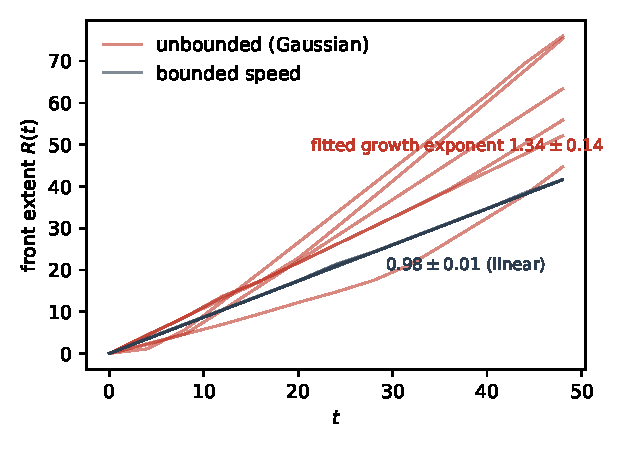
\includegraphics[width=.62\textwidth]{figs/fig1_front_dichotomy.pdf}
\caption{Front dichotomy (experiment E5): front extent $R(t)$ for unbounded
(Gaussian) versus bounded velocity laws, six runs each. Reproduce:
\texttt{python3 src/wake\_r/paper\_figs.py} (data:
\texttt{data/phase\_r/E5\_front.json}).}
\label{fig:front}
\end{figure}

\subsection{The convention dichotomy}
Does motion help colonization? Theorem~D answers ``yes, decisively'' for the
entry-driven convention, and experiment E4c confirms strict monotonicity of
survival probability in the velocity scale ($0.73\to0.91$ over
$\sigma\in[0,0.16]$ at fixed $\rho,p$). But replace fire-and-forget with a
\emph{dwell-time requirement} (transmission requires residence within range
for a fixed time) and the answer inverts: experiment E7 exhibits a
non-monotone survival curve with an optimal speed $\sigma^*\approx0.4$
(survival fraction $0.06\to0.31\to0.00$), consistent with the optimal-velocity
phenomenology observed in mobile-agent epidemic models
\cite{peruanisibona,rodriguez19}. \emph{The answer to ``does motion help''
is a function of the transmission convention}, exhibited here within a
single model family (Figure~\ref{fig:dichotomy}). A related trio of
non-monotonicities (in particle number, in re-marking, in timing --- all
SIR-type interference effects) is recorded in the method archive.

\begin{figure}[t]\centering
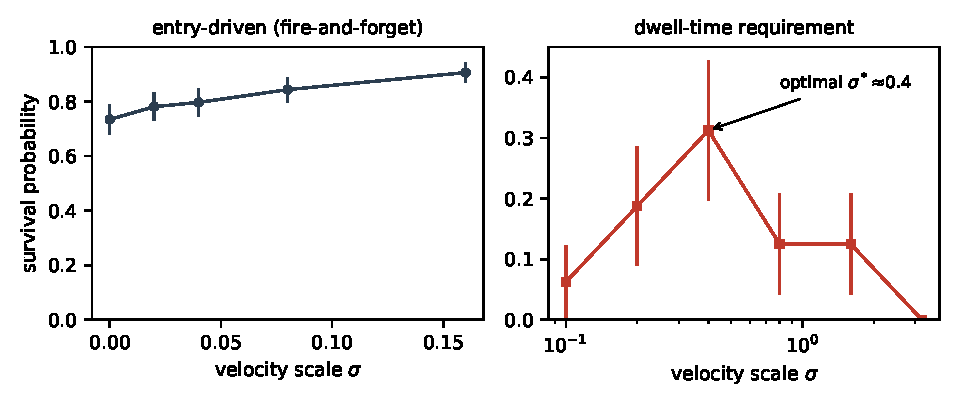
\includegraphics[width=.95\textwidth]{figs/fig2_convention_dichotomy.pdf}
\caption{Convention dichotomy (experiments E4c, E7): survival probability
versus velocity scale $\sigma$. Left: entry-driven fire-and-forget ---
monotone increasing. Right: dwell-time requirement --- optimal speed
$\sigma^*\approx0.4$. Error bars are binomial standard errors. Reproduce:
\texttt{python3 src/wake\_r/paper\_figs.py} (data:
\texttt{data/phase\_r/\{E4c\_dip,E7\_dwell\}.json}).}
\label{fig:dichotomy}
\end{figure}

%======================================================================
\section{Verification: method and boundary}\label{sec:verification}

Every mathematical claim above was developed under a claim-driven protocol
with three layers: (i) an independent simulation device (analytic
closest-approach entry detection, time-step independent) used to attempt
numerical falsification of every stated claim; (ii) adversarial,
line-by-line review of each completed proof by fresh AI instances sharing no
context with the author system --- Theorem~C2 passed on the eleventh cycle,
and the complete cycle ledger, including more than ten caught errors (five
geometric-arithmetic, one non-convexity, one tube-direction, one
normalization-bridge gap, one exposure-length gap, one over-general lemma),
is disclosed in Appendix~B; (iii) machine certification, by interval
arithmetic, of every geometric constant of the survival proof, including the
normalization bridge (Appendix~A). All bibliography entries carry an arXiv
identifier or DOI and were mechanically resolved by the verification script
of Appendix~A; the resolution log is included in the bundled repository
archive (\texttt{wake-repo-v1.tar.gz}).

\textbf{Boundary.} This internal verification --- independent AI review
instances plus machine certification --- \emph{is not a substitute for human
peer review}. The role of AI systems in this work, and the exact experimental
conditions under which the mathematics was produced (including the empty
steering-intervention log), are disclosed in Appendix~B, which also serves
as the AI-use disclosure in the sense of current arXiv policy. The author
takes full responsibility for all content.

%======================================================================
\section{Open problems}\label{sec:open}

\begin{enumerate}
\item \textbf{Pure isotropy.} Remove the bounded-density hypothesis
($\relL$) from Theorem~C2.
\item \textbf{Threshold separation.} Does the full model survive anywhere
inside $r(K)<1$? (The reverse channel breaks the branching \emph{bound};
whether it moves the \emph{threshold} is open.)
\item \textbf{Repaired full-model extinction.} An extinction condition for
the full model incorporating the reverse channel into the transfer kernel;
without additional assumptions this appears hard (Appendix~B, cycle~4).
\item \textbf{Velocity monotonicity (C4).} Pathwise coupling monotonicity of
survival in the velocity scale for the entry-driven model; open, in line
with neighbouring open problems \cite{ks05,linkerremenik}. The
non-monotonicity trio shows naive couplings must fail.
\item \textbf{Front shape theorem.} Existence of the limiting front shape
and speed for bounded $\nu$; explicit constants for $C_0$ and critical
exponents.
\end{enumerate}

\section*{Acknowledgements}
The mathematical exploration, proofs, and their revisions were carried out
by AI systems (Claude Code, model Claude Fable 5) under the verification
protocol of Section~\ref{sec:verification}, with the human author acting as
arbiter (go/stop/harvest rulings and encouragement only; the
steering-intervention log is empty). See Appendix~B for the complete
disclosure.

%======================================================================
\appendix

\section{Machine certification bundle}\label{app:cert}

\subsection{Contents}
The complete repository snapshot is bundled with this Zenodo record as
\texttt{wake-repo-v1.tar.gz} (all version-tracked files at the release
commit; regenerate with \texttt{git archive}). It contains:
\texttt{src/wake\_r/geo\_verify.py} (certifying verifier, version~6;
deterministic, standard library only),
\texttt{docs/phase-r/certification-log-v6.txt} (full scan log),
\texttt{src/wake\_r/device.py} (falsification device),
\texttt{src/wake\_r/paper\_figs.py} (figure generation),
\texttt{data/phase\_r/*.json} (experiment archive E1--E8c), and
\texttt{scripts/verify\_refs.py} with its resolution log (bibliography
verification). Reproduction: \texttt{python3 src/wake\_r/geo\_verify.py}.

\subsection{Design}
All proof geometry is certified by interval arithmetic: every perturbation
(parent position within core plus rounding, parent velocity within the
$\pm0.05\wbar$ cover, entry offset $\le R$, window sweep, branch signs,
target rounding) is propagated as component intervals; Euclidean norms are
bounded by the exact closed forms
$\min\|x\|^2=\sum_i\mathrm{dist}(0,[l_i,h_i])^2$ and
$\max\|x\|^2=\sum_i\max(l_i^2,h_i^2)$; the window sweep uses a $4096$-cell
grid with a Lipschitz penalty
$|\partial_s w_{\mathrm{req}}|\le(\sup|v_p|+\sup|w_{\mathrm{req}}|)/(\Tg-\Ta)$
and the conservative left endpoint for $h_0$. The bridge certification
computes the acceptance mass $\frac{1}{200}\cdot\frac{1-\cos\theta^*}{2}$
and the disclosed mass via the exact box--ball Steiner volume and the
site-count series $\frac{\sqrt3}{8}\zeta(2)+(1+\mathrm{diam}\,
\mathcal{K}/8a)\zeta(3)$, with the worst shell endpoint taken separately on
each side. All approximations are monotone in the conservative direction;
the box-hull correctness is the direct inclusion
$\bigcup_v\mathcal{K}(v)\subseteq B(0,2R)\oplus H_1\oplus(-H_2)$.

\subsection{Certified table (excerpt)}
\begin{center}
\begin{tabular}{rrrrrr}
\toprule
$K_0$ & $\tau/\Ts$ & slack$/\wbar$ & bad ($\relL{=}1$) & accepted & $\relL_{\max}$\\
\midrule
20 & 0 & $+0.00483$ & $1.688\times10^{-9}$ & $2.640\times10^{-8}$ & $\mathbf{7.82}$\\
20 & 1 & $+0.00536$ & $2.100\times10^{-10}$ & $3.253\times10^{-8}$ & $77.47$\\
20 & 3 & $+0.00562$ & $2.618\times10^{-11}$ & $3.583\times10^{-8}$ & $684.33$\\
24 & 0 & $+0.00499$ & $1.091\times10^{-9}$ & $2.821\times10^{-8}$ & $12.93$\\
\bottomrule
\end{tabular}
\end{center}
Verdict: $K_0=20$, $\relL\le4$, $\Ta=\Ts/32$ --- PASS (bridge and geometry),
with margin factor $\approx1.95$ over the assumed $\relL\le4$. For
comparison, the pre-repair configuration $K_0=5$ yields
$\relL_{\max}=0.03$: the bridge genuinely fails there, exactly as found in
review cycle~10 (Appendix~B). Independent reproductions of these numbers by
fresh review instances are recorded in Appendix~B.

\section{Method record (self-contained)}\label{app:method}

\emph{This appendix is a self-contained disclosure document; it can be read
independently of the main text. It records the experimental conditions under
which the mathematics of this paper was produced: the protocol separating
encouragement from mathematical steering, the (empty) intervention log, the
complete review-cycle ledger with all caught errors, and the evolution of
the machine-verification layer.}

\subsection{Design}
The executor (an AI system: Claude Code, model Claude Fable 5) held full
authority over mathematical exploration --- proof strategies, experiment
design, retraction decisions. The human author acted solely as arbiter
(go/stop/harvest rulings) and encourager; an independent AI chat instance
relayed verification verdicts only. Claim-driven verification: on every
declared claim, (i) numerical falsification against an independently
implemented simulation device, (ii) literature check; on every completed
proof, line-by-line adversarial review by a \emph{fresh} AI instance sharing
no conversational context, one new instance per cycle.

\subsection{Steering protocol and intervention log}
Permitted interactions: encouragement, confidence, generic advice
(``stepping away is allowed''), and the go/stop/harvest ruling. Forbidden:
mathematical hints, literature pointers, evaluations of proof directions.
Any steering intervention was to be logged as a change of experimental
conditions. \textbf{The intervention log is empty}: from sprint start
(2026-08-15) to close (2026-08-16), no forbidden intervention occurred; all
human inputs were start permissions, encouragement, and rulings.

\subsection{Review-cycle ledger}
\begin{center}
\footnotesize
\begin{tabular}{clp{3.1cm}p{6.9cm}}
\toprule
\# & target & verdict & errors caught / outcome\\
\midrule
self & Thm.~A v1 & self-rejected & chain factors share velocities; scalar $\bar m^k$ invalid $\to$ spectral $r(K)$\\[1pt]
1 & Thm.~A/C6a & accepted after fix & window quantification gap $\to$ deterministic attempt-time recursion\\
2 & C2 v1 & rejected & empty landing set; co-moving particles break finite range; no thinning monotonicity\\
3 & C2 v2 & core isolated & D-separation impossible; general memoryless lemma false (negative-information)\\
4 & A-full & \textbf{retracted (false)} & reverse-channel counterexample $\to$ device-certified $4.4\sigma$; became Section~\ref{sec:afull}\\
5--8 & C2 v3--v6 & partial accepts & five geometric-arithmetic errors; $\|w\|$ non-convexity $\to$ interval arithmetic\\
9 & C2 v7 & remanded & tube direction (relative velocity); honest Minkowski sums fail $\to$ window shortening\\
10 & C2 v8 & \textbf{incomplete} & normalization bridge missing (real: $33$--$440\times$ short); exposure-length gap\\
11 & C2 v9 & \textbf{accepted} & over-general sector lemma $\to$ replaced by box-hull Steiner; numbers reproduced\\
spot & box-hull, Thm.~D & accepted & scale-invariance lemma made explicit; false ``superset'' justification removed\\
C6b & Prop.~C6b & accepted (minor) & tightened to $\lfloor t/\tau\rfloor$; well-foundedness made explicit\\
\bottomrule
\end{tabular}
\end{center}
Tally: more than ten errors caught; two became discoveries (reverse channel,
non-monotonicity trio), one became a strengthening (window shortening); one
theorem retracted and re-cast as a correct impossibility statement
(Section~\ref{sec:afull}, with the claim strength corrected in final
editing: what is proved is that the branching-type bound does not extend,
not that the thresholds separate).

\subsection{Machine-verification evolution}
Monte-Carlo minimum (rejected in review: not a worst-case proof) $\to$
corner enumeration with Lipschitz penalties (rejected: anti-conservative on
concave directions of the norm) $\to$ interval arithmetic with exact norm
bounds and bridge certification (final; also caught two design errors before
they reached review). Operational conclusion: \emph{every geometric constant
of a proof of this kind should be machine-certified}; hand-computed geometry
failed five times in review.

\subsection{Disclosure statement}
The mathematical content of this paper (formulations, proofs, retraction
decisions included) was explored by an AI executor; verification used the
three layers above. The human author's role was direction-level arbitration
and encouragement; the steering log is empty. This internal verification is
not a substitute for human peer review; the reader and referee should treat
this record, including the error ledger, as the disclosure of the
verification boundary.

\section{Proof details}\label{app:proofs}

\subsection{Theorem A}
[Full computation: capsule volume lemma; multivariate Mecke over
time-ordered chains; deterministic attempt-time recursion
$t_j=\max(\inf T_j,t_{j-1}+\tau)$; operator power bound
$\E[\#\text{chains of length }k]=\langle\mathbf{1},K^k\mathbf{1}\rangle$
with equality; summability under $r(K)<1$ and a.s.\ extinction of the SIR
variant. As accepted in review cycle 1; the full text follows the record in
the bundled repository archive (\texttt{wake-repo-v1.tar.gz}), file
\texttt{docs/phase-r/claims.md}.]

\subsection{Theorem B}
As in Section~\ref{sec:thmB}; the event identification is elementary given
the single-interval property and instant attempts at marking times.

\subsection{Theorem C2}
The complete proof in its accepted form (review cycle 11 plus accepted
wording fixes) follows the consolidated record
\texttt{docs/phase-r/c2-proof-final.md} in the bundled repository archive
(\texttt{wake-repo-v1.tar.gz}), whose
sections map to: parameters and lattice; the geometry contract (interval
certification); the erosion patch lemma; the disclosure-capsule
identification; the normalization bridge (box-hull Steiner volume, site
count, certified inequality); Lemma X (private-coin coupling: failure
requires a private coin; indicator-path conditioning preserves joint
exponential independence; post-arrival interference is rescue-only);
same-branch flux correction; assembly (sequential conditioning, domination
by product measure, oriented site percolation via Liggett's bound
\cite{liggett95} on the identified lattice, ignition, coverage clause).

\subsection{Theorems C6a and C6b$'$}
C6a: for any speed level $u$, the seed's capsule meets entries of speed
$\ge u$ at positive rate (unbounded $\nu$); with $\Ts=\infty$ marked
carriers of speed $\ge u$ eventually exist for every $u$, so
$\liminf R(t)/t\ge u$ for all $u$. C6b$'$: as in Section~\ref{sec:fronts},
with the exact telescoping travel-time accounting and the well-foundedness
of ancestries from the $\tau$-increments; the bound applies to dead-marked
particles as well since only the speed bound is used after marking.

\subsection{Theorem D}
As in Section~\ref{sec:thmD}, with the scale-invariance lemma: pushing
$\nu^0$ forward under $w\mapsto sw$ maps the shell $S^0$ to $sS^0$,
preserves the shell mass $q$, and multiplies the density by $s^{-3}$ and
the shell volume by $s^3$, so $\relL$ is invariant; $\Kmix$ and $m_1$ scale
linearly in $s$ at fixed $\tau/\Ts$.

\bibliographystyle{plain}
\bibliography{refs}

\end{document}
